\documentclass[11pt]{article}

% basic packages
\usepackage[margin=1in]{geometry}
\usepackage[pdftex]{graphicx}
\usepackage{amsmath,amssymb,amsthm}
\usepackage{custom}
\usepackage{lipsum}

% page formatting
\usepackage{fancyhdr}
\pagestyle{fancy}

% \renewcommand{\sectionmark}[1]{\markright{\textsf{\arabic{section}. #1}}}
% \renewcommand{\subsectionmark}[1]{}
\lhead{\textbf{\thepage} \ \ \nouppercase{\rightmark}}
\chead{}
\rhead{}
\lfoot{}
\cfoot{}
\rfoot{}
\setlength{\headheight}{14pt}

\linespread{1.03} % give a little extra room
\setlength{\parindent}{0.2in} % reduce paragraph indent a bit
\setcounter{secnumdepth}{2} % no numbered subsubsections
\setcounter{tocdepth}{2} % no subsubsections in ToC

\begin{document}

% make title page
\thispagestyle{empty}
\bigskip \
\vspace{0.1cm}

{\fontsize{18}{18} \selectfont \bf \sffamily Result Reproduction}

% main content
\section{Goncalves et al., ``Numerical solution of the time dependent Ginzburg-Landau equations for mixed (d + s)-
wave superconductors"}

We try to reproduce section VIII, the paper's computational results. 
The parameters are $\kappa_D = 2, \tau_1=8/3, \tau_3=16/3, \tau_4=2, \nu=-2, \eta_s=2, \eta_v=1$. Note that these correspond to microscopically derived coefficients from other papers. The square film has dimensions $8\xi_D$ x $8\xi_D$.
The grid starts off with (everywhere) $\psi_D=1$, $\psi_S=0$, $\v{B}=0$. In the paper, they gradually sweep the field up to $2.5H_{c2}$ and back down to $0$.
My computer only had the capability to step in intervals of $0.5H_{c2}$, which probably accounts for the differences in behavior below. Another possibility is that solving on a mesh rather than a grid causes differences, but I think that's less likely.

\begin{figure}[htbp]
    \centering
    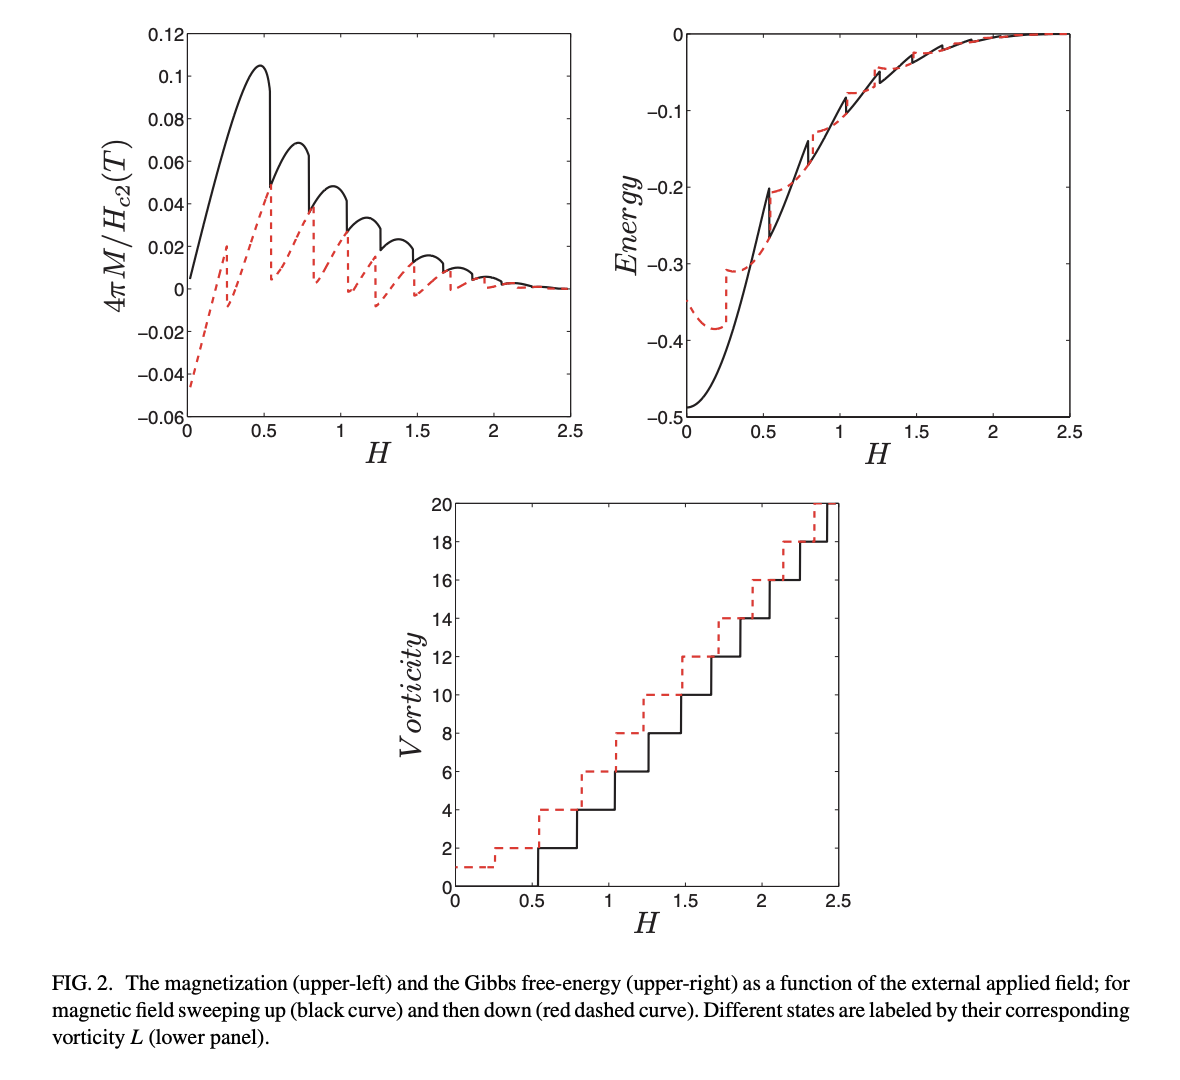
\includegraphics[width=0.55\textwidth]{images/goncalves_fig2.png}

    \vspace{0.5em}

    \begin{minipage}[t]{0.49\textwidth}
        \centering
        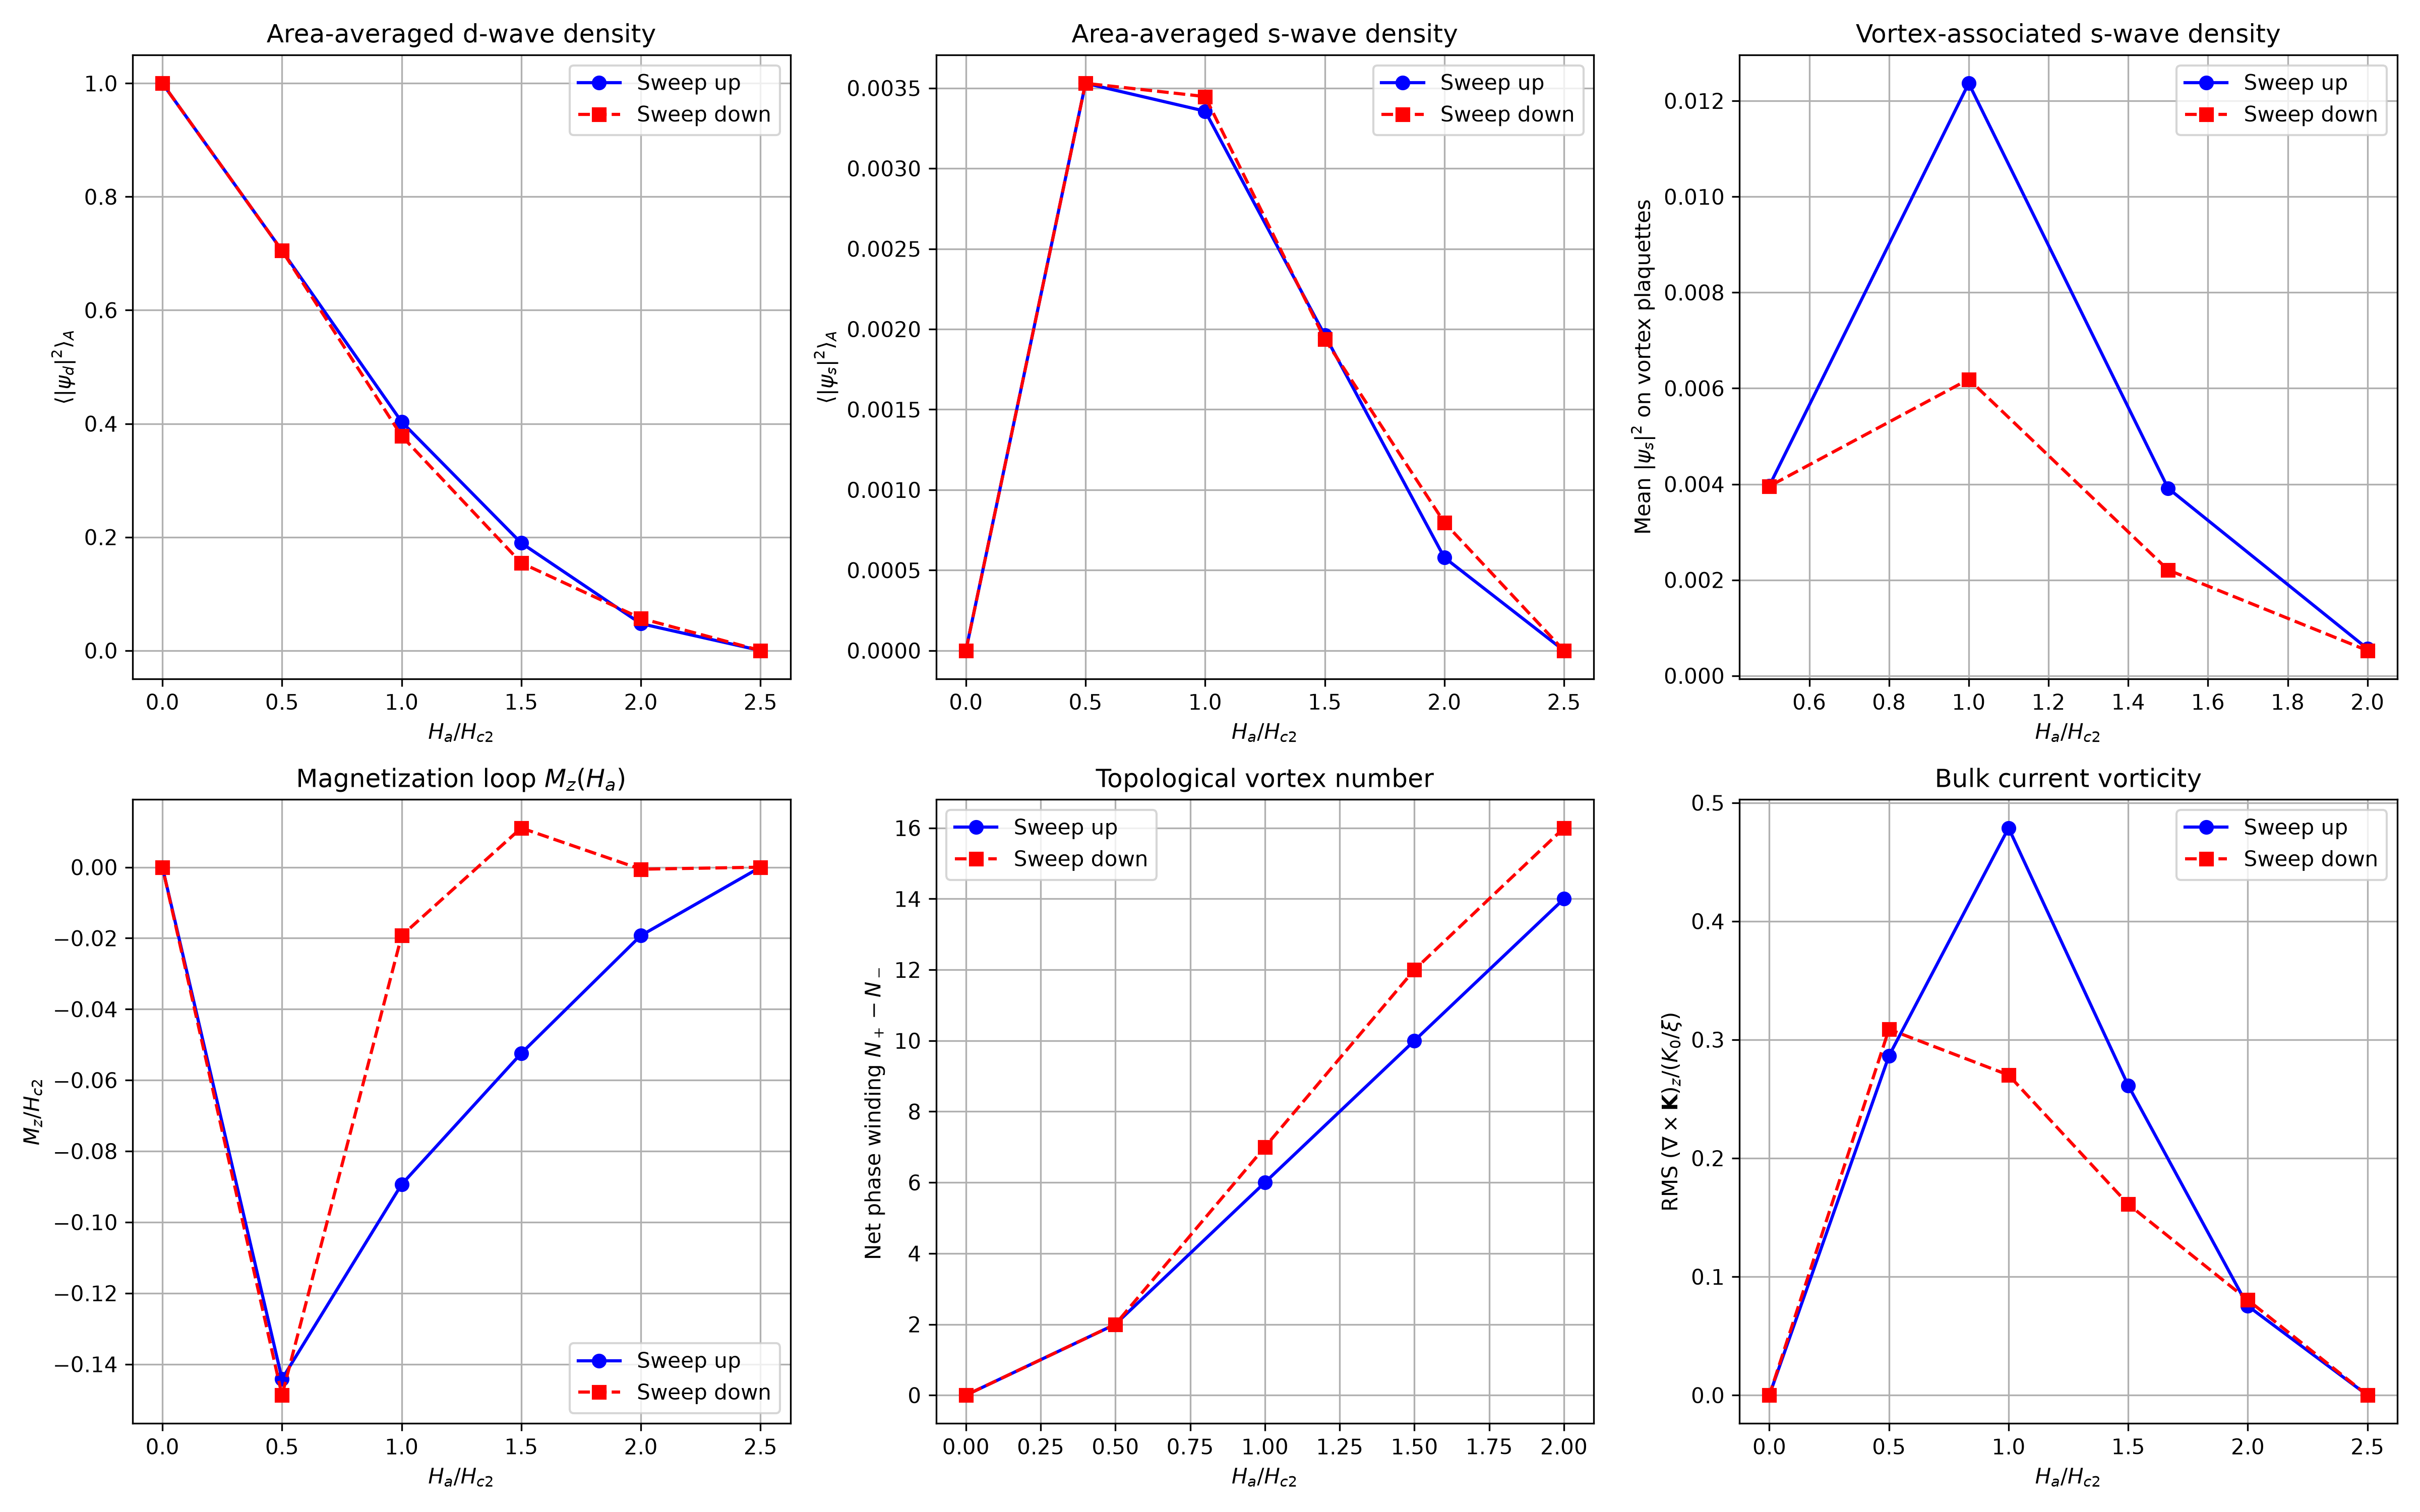
\includegraphics[width=\linewidth]{images/goncalves_reprod_h_dependence.png}
    \end{minipage}\hfill
    \begin{minipage}[t]{0.49\textwidth}
        \centering
        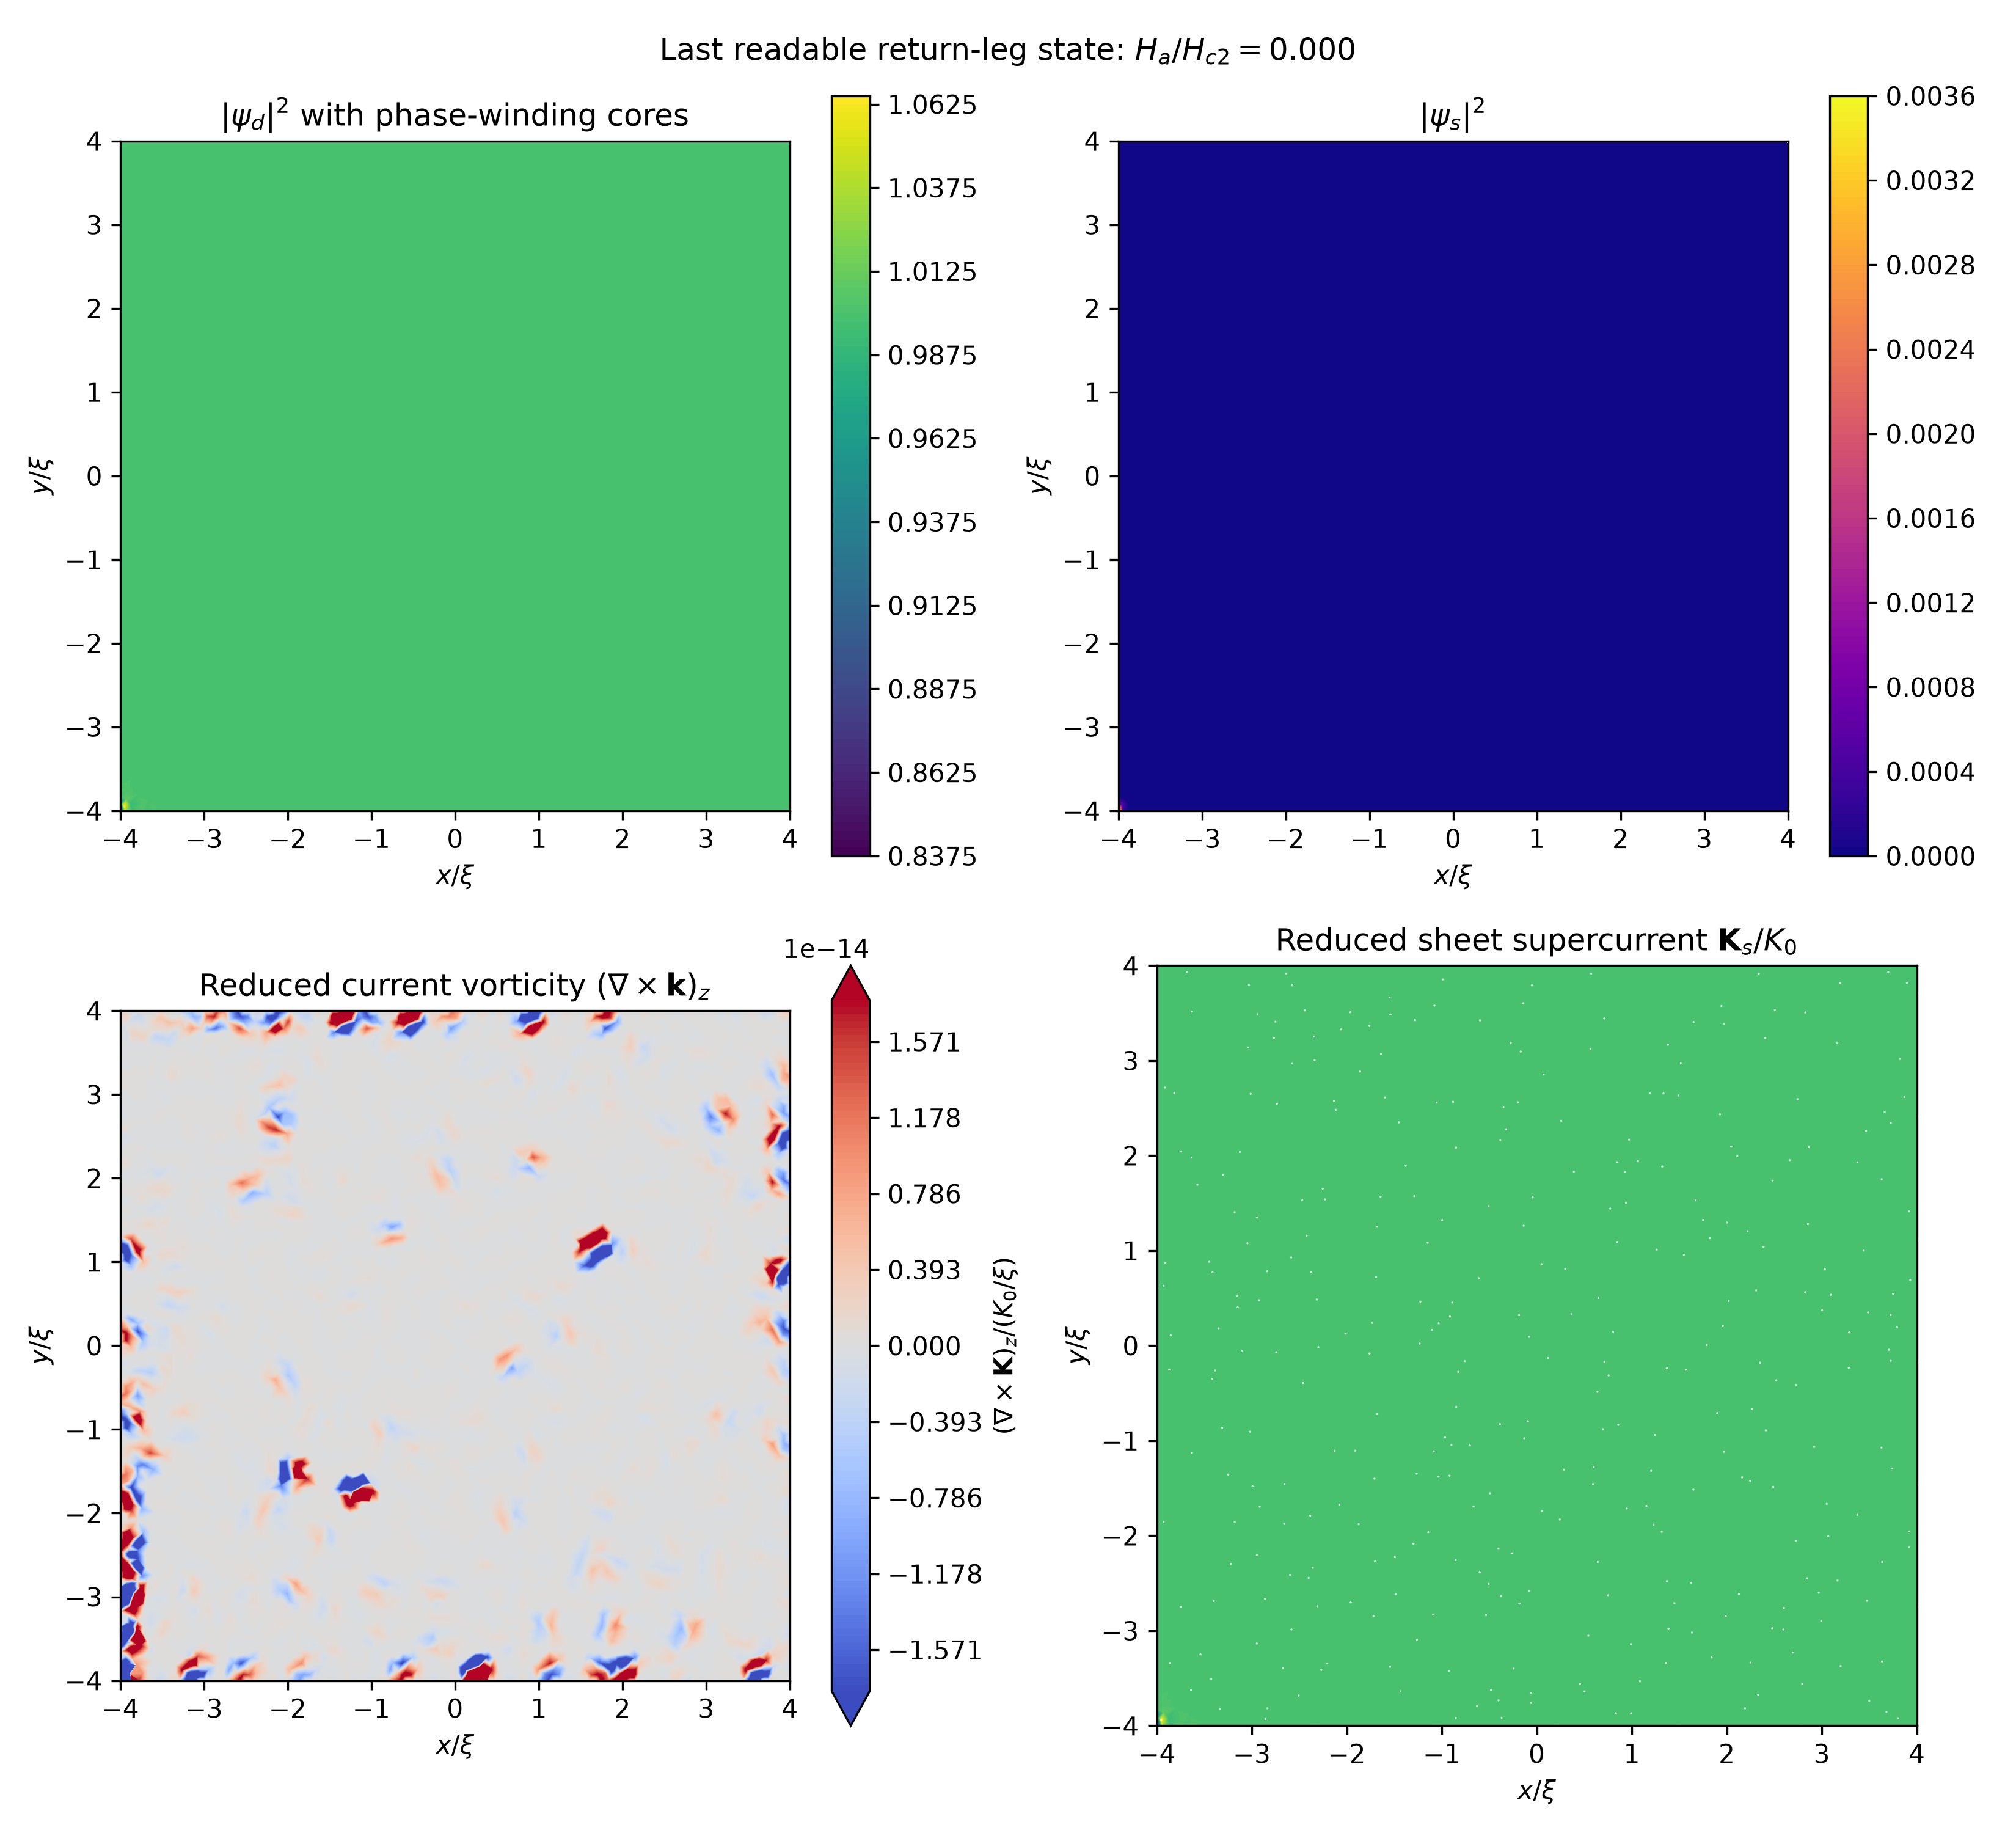
\includegraphics[width=\linewidth]{images/goncalves_reprod_trapped_flux.png}
    \end{minipage}
\end{figure}

One issue, among many other differences (due to my intervals), is that there is no vortex remaining when the system gets back to $H = 0$. However, the vortex count seems to roughly track otherwise.

\begin{figure}[htbp]
    \centering
    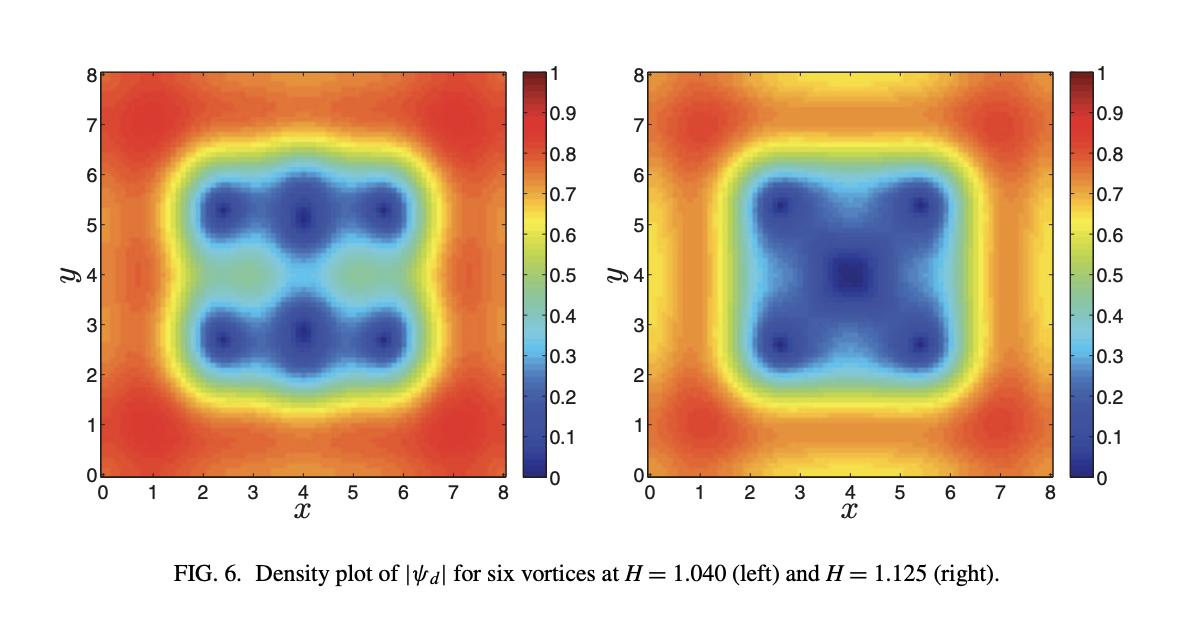
\includegraphics[width=0.85\textwidth]{images/goncalves_fig6.png}

    \vspace{0.5em}

    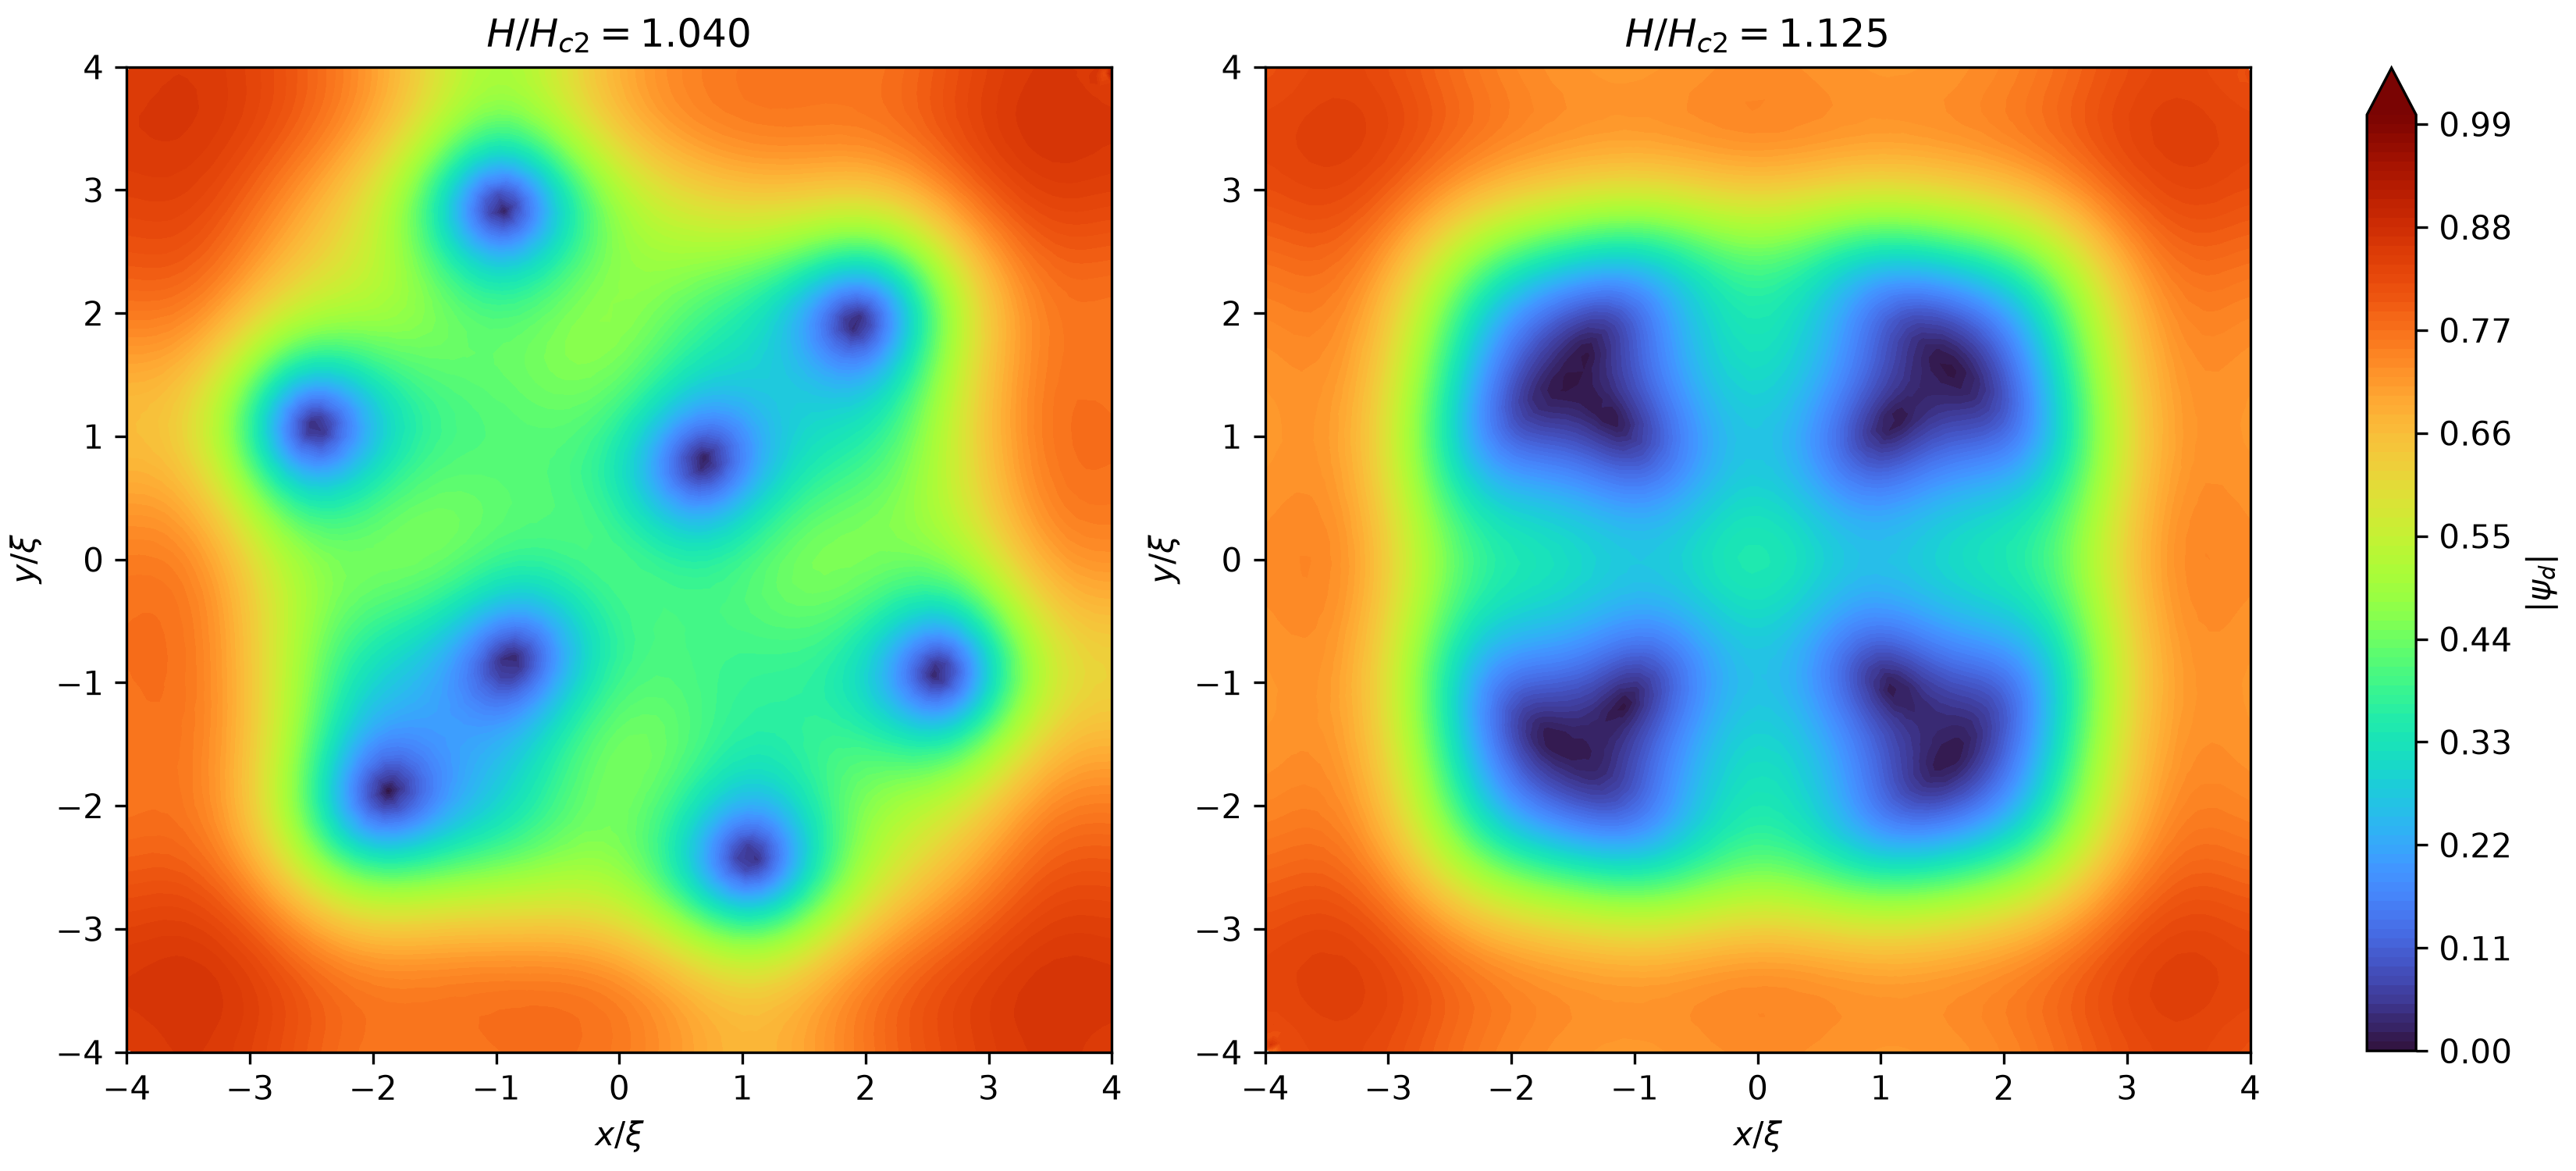
\includegraphics[width=0.8\textwidth]{images/goncalves_reprod_d_wave_H_1.040_1.125.png}
\end{figure}

I tried to reproduce these plots by going straight from $H=0$ to the desired values, but again hysteresis seems to cause behavioral differences (in mine there are 8 vortices rather than 6).

\section{Xu, Ren, Ting, ``Structures of single vortex and vortex lattice in a d-wave superconductor"}



\section{Lin et al., ``Distinguishing between s+id and s+is pairing symmetries
in multiband superconductors through spontaneous
magnetization pattern induced by a defect"}

\section{Lei et al., ``Field Driven Pairing State Phase Transition
in $d_{x^2-y^2} + id_{xy}$-Wave Superconductors"}

\end{document}
